\documentclass{article}

% if you need to pass options to natbib, use, e.g.:
% \PassOptionsToPackage{numbers, compress}{natbib}
% before loading nips_2016
%
% to avoid loading the natbib package, add option nonatbib:
% \usepackage[nonatbib]{nips_2016}

\usepackage[final]{nips_2016}

% to compile a camera-ready version, add the [final] option, e.g.:
% \usepackage[final]{nips_2016}

\usepackage[utf8]{inputenc} % allow utf-8 input
\usepackage[T1]{fontenc}    % use 8-bit T1 fonts
\usepackage{hyperref}       % hyperlinks
\usepackage{url}            % simple URL typesetting
\usepackage{booktabs}       % professional-quality tables
\usepackage{amsfonts}       % blackboard math symbols
\usepackage{nicefrac}       % compact symbols for 1/2, etc.
\usepackage{microtype}      % microtypography
\usepackage{graphicx}
\usepackage{subcaption}
\usepackage{listings}
\usepackage{color}

\definecolor{deepblue}{rgb}{0,0,0.5}
\definecolor{deepred}{rgb}{0.6,0,0}
\definecolor{deepgreen}{rgb}{0,0.5,0}
\definecolor{mygreen}{rgb}{0,0.6,0}

\DeclareFixedFont{\ttb}{T1}{txtt}{bx}{n}{7} % for bold
\DeclareFixedFont{\ttm}{T1}{txtt}{m}{n}{7}  % for normal

\lstset{ 
otherkeywords={name, shape, dtype, initializer, value, filters, stride, padding},
breaklines=true,
tabsize=1,
language=Python,
basicstyle=\ttm,
commentstyle=\color{mygreen},
keywordstyle=\ttb\color{deepblue},
stringstyle=\color{deepgreen},
showstringspaces=false,
emphstyle=\ttb\color{deepred},
keepspaces=false
}  

\title{Prediction of Protein Secondary Structure using Convolutional Neural Networks (CNN)}

% The \author macro works with any number of authors. There are two
% commands used to separate the names and addresses of multiple
% authors: \And and \AND.
%
% Using \And between authors leaves it to LaTeX to determine where to
% break the lines. Using \AND forces a line break at that point. So,
% if LaTeX puts 3 of 4 authors names on the first line, and the last
% on the second line, try using \AND instead of \And before the third
% author name.

\author{
  Simon B. Jensen\\
  Software Development \& Technology\\
  IT University of Copenhagen\\
  \texttt{sije@itu.dk} \\
  %% examples of more authors
  %% \And
  %% Coauthor \\
  %% Affiliation \\
  %% Address \\
  %% \texttt{email} \\
}

\begin{document}
% \nipsfinalcopy is no longer used

\maketitle

\section{Introduction}
\label{sec:introduction}
To design medicine for specific anomalies in the DNA of living organism it is useful to know the 3D structure of the protein which, due to the anomaly in the DNA or some mutation, is modified. When we talk about the structure of proteins, four different structure levels are mentioned. The primary-, secondary-, tertiary- and quaternary structure. In this paper we focus on the primary- and secondary structure (SS). More specifically we will focus on using Convolutional Neural Networks (CNNs) for predicting the secondary structure of proteins given their primary structure. The tertiary structure is however particularly interesting as it describes the 3D structure of the protein molecule, which reveals very important functional and chemical properties, such as which chemical bindings the protein can take part in. The plan for the actual Master thesis project was therefore initially to research on the use of deep learning for predicting the tertiary structure of proteins given their secondary structure. But this initial plan changed due to a sudden Master thesis project opportunity at Daimler AG in Ulm, Germany, which arose half way through the semester. The project at Daimler AG has the head line: ``Deep learning for learning Autonomous vehicles to navigate in bad weather condition'', and it will be focusing on investigating neural network architectures and developing and utilizing deep neural networks for autonomous vehicles. The work carried out in this thesis preparation project is however neither wasteful or made in vain, as it gives good insights in concepts of deep learning and important familiarity with ML frameworks.     

\section{Work carried out so far} 
During the Thesis preparation course the following work has been carried out:
\begin{enumerate}
\itemsep0em 
\item Implementation of a CNN, in the Tensorflow framework, for predicting protein secondary structures using the CullPDB data set.
\item Implementation of a CNN, in the ML framework Caffe, for classifying images of digits between 0-9 using the MNIST data set.
\end{enumerate}

The work described in (1) achived a prediction accuracy of $\sim$81\% for 3-state SS prediction on the CullPDB data set (more on this in section \ref{sec:protein-structures} and \ref{sec:experiments}). The work described in (2) was carried out as part of the interview process at Daimler AG. It was a requirement to implement the CNN in Caffe for this task, due to the fact that the DENSE project (aDverse wEather eNvironmental Sensing systEm) at Daimler uses primarily this framework. Using a LeNet-5 based CNN architecture it is easily achiveable to reach ~98 \% prediction accuracy on one of the most famouse data sets for benchmarking ML models on, the MNIST data set.

\section{Protein Structures and Protein Data}
\label{sec:protein-structures}
In order to implement a CNN for predicting proteins secondary structure from their  primary it is necessary to have at least a minimal degree of knowledge about the composition of proteins. Though certain deep learning architectures are actually able to extract low level features in the data by themself, extracting mid- and high level features require an expert degree of domain knowledge. As this project is ment as a preparation and learning experience we will focus on just the basics. The following section is a brief description of protein primary- and secondary structure and of the CullPDB data set, which was used for training, testing and validation during the project.  

The primary structure of proteins are described by the sequence of amino acids on their polypeptide chain, also know as the protein's profile. There are 20 natural occuring amino acids which, in a one letter notation, is denoted by: 'A', 'C', 'D', 'E', 'F', 'G', 'H', 'I', 'K', 'L', 'M', 'N', 'P', 'Q', 'R', 'S', 'T', 'V', 'W', 'Y'. 'A' standing for Alanine, 'C' for Cysteine, 'D' for Aspartic Acid etc. For the full list see \footnote{https://en.wikipedia.org/wiki/Protein\_primary\_structure}. A 21. letter, 'X', is sometimes used for denoting an unknown or any amino acid. In the CullPBD data set the first 22 out of 57 features of each amino acide are indicating whether the amino acid data point is one of the 20 natural occuring amino acids, whether it's the unknown/any amino acid (which was denoted by the 'X') or whether it's a 'No Seq'. Where 'No Seq' means that the data point is no longer part of the peptide chain. In order words we have reached the end of the protein. 

A protein's polypeptide chain typically consist of around 200-300 amino acids, but it can consist of far less or far more. The amino acids can occure at any position in a chain, meaning that even for a chain consisting of 4 amino acids, there are $20^4$ possible distinct combinations. In the CullPDB data the average protein chain cosists of 208 amino acids. The chains are however described by a $700\times57$ vector to keep the data size consistent. The 700 denotes the peptide chain and the 57 denotes the number of features in each amino acid. When the end of a chain is reached the rest of the vector will simply be labeled as 'No Seq'. 

Proteins' secondary structure determines structural states of local segments of amino acid residues in the protein. The alpha-helix state for instance forms a coiled up shape and the beta-strand forms a zig-zag like shape etc. The secondary structure of the protein is interesting because it, as mentioned in the introduction, reveals important chemical properties of the protein and because it can be used for further predicting it's tertiary structure. When predicting proteins' secondary structure we distinguish between 3-state SS prediction and 8-state SS prediction. For 3-state prediction the goal is to classify each amino acid into either:

\begin{itemize}
\item alpha-helix, which is a regular state denoted by an 'H'
\item beta-strand, which is a regular state denoted by an 'E'
\item coil region, which is an irregular state denoted by a 'C' 
\end{itemize}

Protein 3-state SS prediction can be viewed as a more coarse-grained task than 8-state SS prediction, as 8-state prediction is more challenging but also reveals more structural details than 3-state prediction. The scope of this project has been narrowed down to 3-state SS prediction. The letters which denotes the above secondary structures are not to be confused with those which denotes the amino acids. For 8-state prediction, Alpha-helix is further sub-divided into three states: alpha-helix ('H'), $3_{10}$ helix ('G') and pi-helix ('I'). Beta-strand is sub-divided into: beta-strand ('E') and beta-bride ('B') and coil region is sub-divided into: high curvature loop ('S'), beta-turn ('T') and irregular ('L'). 

\subsection{CullPDB data set}
We already mentioned the CullPDB data set, but in detail it's a data set consisting of $6133$ proteins each of $39900$ features. The $6133$ proteins $\times39900$ features can be reshaped into $6133$ proteins $\times700$ amino acids $\times57$ features. For preprocessing and reshaping the CullPDB data set a script kindly provided by Jes Frellsen and Wouter Boomsma was used. The script splits the data into input data of shape $n\times700\times44$ ($n$ being the number of proteins) for a training-, testing- and validation set and corresponding labels of shape $n\times700\times4$. During the project $\sim5000$ proteins are used for training corresponding to approximately 80\% of the data, $\sim600$ are used for testing and $\sim550$ are used as validation set corresponding to $\sim$10\% for each. As it should be noted only $48$ of the $57$ available features are used ($44$ for the input data and $4$ for the labels). A detailed describtion of the features can be found at \footnote{http://www.princeton.edu/$\sim$jzthree/datasets/ICML2014/dataset\_readme.txt}. 

\begin{table}[t]
  \label{table:distribution}
  \centering
  \begin{tabular}{lll}
    \toprule
    SS-state     & Occurences     & \% of total \\
    \midrule
    Alpha-helix & 489786 & $38.3$     \\
    Beta-strand & 291314 & $22.8$     \\
    Coil region & 497234 & $38.9$     \\
    \bottomrule
    Total 		& 1278334 & $100$ \\
  \end{tabular}
  \caption{Distribution of alpha-helix, beta-strand and coil region states in the CullPDB data set}
\end{table}

In the data set the distribution of 3-state secundary structures are shown in table \ref{table:distribution}. Optaining a prediction rate of around 40 \% should therefore be considered a absolute minimum, as it would be possible for even a simple program which randomly picks alpha-helix or coil region as the label for each amino acid to optain this.   

\section{Convolutional Neural Network}
\label{sec:convolutional}
Convolutional Neural Networks (CNNs) are a class of neural networks which in recent years have proven very useful and succesful in diverse fields suchs as object detection, image classification, protein structure prediction amongst others. The secret behinde CNNs success are their ability to capture information in input space between neighbouring or nearby data points e.g. adjacent pixels in images or adjacent amino acids residuals in poly peptide chains. CNNs could in principle prove useful in any field where nearby data points in input space are somehow correlated. A known problem encountered in protein SS prediction, which can not be captured by conventional CNNs, is the fact that some beta-strand states are stabilized by hydrogen bond formed with other beta-strands which can be far away from each other in the protein chain. This problem is described in [1]. In this section we describe the CNN implementation of this project which was used for 3-state protein SS prediction.       

\subsection{Implementation}
The architecture of the CNN consists of the following layers:
\begin{itemize}
\item An input layer of size: \textit{batch size} $\times700\times44$. 
\item A convolutional layer (A $1\times11$ kernel with $44$ input channels and $88$ output channels. Stride is set to $1$ and the padding algorithm is set to 'SAME') 
\item A rectified linear unit activation function (This layer will remove all negative values)
\item A convolutional layer (A $1\times11$ kernel with $88$ input channels and $44$ output channels. Stride is set to $1$ and the padding algorithm is set to 'SAME') 
\item A rectified linear unit activation function (This layer will remove all negative values)
\item A convolutional output layer (A $1\times11$ kernel with $44$ input channels and $4$ output channels. Stride is set to $1$ and the padding algorithm is set to 'SAME') 
\end{itemize}  

Convolutional layers are kernels (sometimes referred to as filters) of a certain size which are moved along the input matrix according to the stride value. In our case, the size of the kernel for each of the three convolutional layers is a $1\times11$ kernel. In  [2] it is stated that the average length of an alpha-helix is around 11 residues, which is the reason why they use 1x11 kernels for each of their convolutional layers. 

The stride in our network is set to 1, meaning that the kernels are moved a single column at a time in the input data matrix. The out-channel is the number of different kernels we try moving along the input data matrix, which each will create an output matrix which is further passed along in the network. In our case we try out 88 different kernels in the first convolutional layer, 44 in the second and only 4 in the final layer. In theory, each different kernel should be able to capture a different feature from the input, but it will also add to the complexity and size of the network and the total training time required. 

The following code snippet shows how the network is implemented in Tensorflow (The library is imported into python as \textbf{tf}):

\lstinputlisting[language=Python, firstline=113, lastline=130]{code/model.py}

Weights and Biases are given and initialized by the following code snippet:

\lstinputlisting[language=Python, firstline=132, lastline=151]{code/model.py}

The x parameter of the cnn\_model function is a Tensorflow placeholder of size: \textit{batch size} $\times700\times44$. Where the batch size is dynamical, meaning we can run the model with any batch size (given that the data can be held in memory). The padding algorithm is set to 'SAME' meaning that the kernels are fit onto the input matrices all the way to the end eventhough there might not be 11 values to fit onto. A 'VALID' padding algorithm will stop as soon as the kernel is not fit onto all 11 values, which will result in a size decrease of the outputted matrix. 

The values of the convolutional kernels and bias matrices are initialized using the xavier initializer which was introduced in [3]. The xavier initializer is a complex matter, but in brief it utilizes information about the number of units in the network's layers to set the weights and biases to relevant initial values, which are not too big or too small. Thereby decreasing the convergences time.

\subsection{Training}  
The training function is given by the following code snippet:

\lstinputlisting[language=Python, firstline=167, lastline=190]{code/model.py}

Where the loss function is the softmax cross entropy. The output of the network is a $700\times4$ matrix which will be compared to the actual label. The softmax function normalizes and converts the output values to likelyhoods with values between 0-1 for each 3-state SS plus the 'No Seq' label. Before each epoch the training data is shuffled, so that we avoid that the model will be starting to learn the order in which the data is fed, but rather learn patterns in the data, no matter which order it's given.

For calculating prediction accuracy, the predicted output of the network is converted to one-hot vectores and compared one by one to the true labels. The prediction accuracy is calculated after each epoch on the part of the data that's assigned for validation, which the model is not being trained on.

We use Tensorflow's Adam optimizer for optimization. In short, the Adam optimizer is a stochastic gradient descent optimizer with an optional decaying momentum parameter. We set the learning rate to $0.002$ and the initial momentum value to the default value $0.9$.

\section{Experiments}
\label{sec:experiments}
The CNN described in \ref{sec:convolutional} is evaluated on it's ability to accurately predict protein 3-state secondary structures. Other architectures were tried out with different kernel sizes and in-/out-channels, but none reaching a better prediction accuracy. The experiments were run for 50 epochs with a batch size of 32 proteins. It would have been interesting to train the model for even more epochs as it wasn't clear whether the model had actually started over-fitting the trianing data after just 50 epochs. But as the experiments were conducted on a hardware limited system running solely on a CPU, even 50 epochs took a few hours. In figure \ref{fig:loss} the softmax cross entropy loss after each epoch is plotted.    

\begin{figure}[t]
\centering
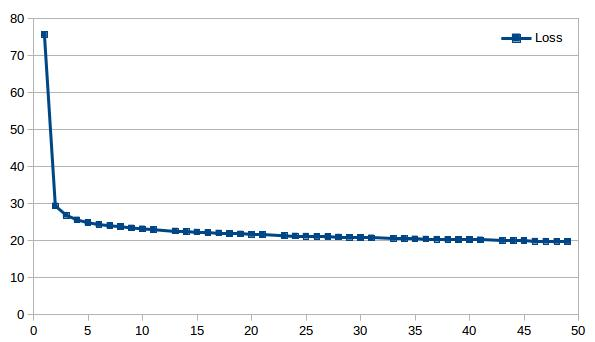
\includegraphics[width=.75\linewidth]{img/loss.jpg}
\caption{The softmax cross entropy loss at epoch 1 to 50}
\label{fig:loss}
\end{figure}

In figure \ref{fig:accuracy} the 3-state protein SS prediction accuracy is shown after each epoch. At around epoch 44 and onwards the prediction accuracy moves up and down sporadically, which could be an indication that the CNN is starting to be overfitted to the training data. The CNN achieved a prediction accuracy of $81,56\%$. For reference, the work conducted in [2], which per January 2016, was the current state of the art achieved a $85.4\%$ prediction accuracy on the CullPDB with a 5-layer Convolutional Neural Fields model.    

\begin{figure}[t]
\centering
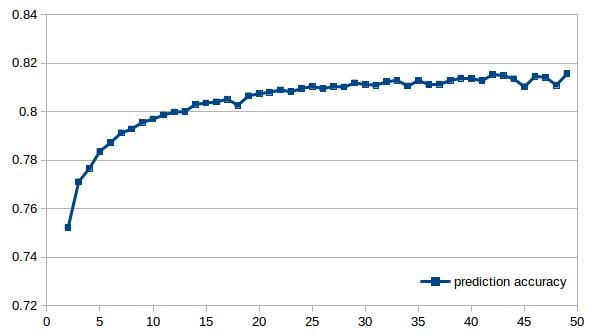
\includegraphics[width=.75\linewidth]{img/prediction-accuracy.jpg}
\caption{The prediction accuracy after 50 epochs}
\label{fig:accuracy}
\end{figure}
  
\section{Future Plan}
The initial plan for the actual Master Thesis project changed half way through the semester. The work carried out doing this Thesis Preparation project which is specific to proteins will not be further followed up on. The work has however given good experience with Tensorflow and Caffe, which will come in handy at Daimler AG. The future plan is, from 1st of September, to move to Ulm, Germany where Daimler's main research department is located. Here I will be working on the, by Daimler, proposed thesis project in cooperation with them and Jes Frellsen. The project has the head line: ``Deep learning for learning Autonomous vehicles to navigate in bad weather condition'', and will be a very small part of the much bigger project, the DENSE project (aDverse wEather eNvironmental Sensing systEm), which is coordinated by Daimler and partly funded by EU  \footnote{http://cordis.europa.eu/project/rcn/203395\_en.html}.        



% STYLE
%The style files for NIPS and other conference information are
%available on the World Wide Web at
%\begin{center}
%  \url{http://www.nips.cc/}
%\end{center}

% LINKS
%\begin{center}
%  \url{https://google.com/protein+secondary+structure/}
%\end{center}

% PARAGRAPHS
%\paragraph{Paragraphs}
%
%There is also a \verb+\paragraph+ command available, which sets the
%heading in bold, flush left, and inline with the text, with the
%heading followed by 1\,em of space.


% CITATIONS
%
%The \verb+natbib+ package will be loaded for you by default.
%Citations may be author/year or numeric, as long as you maintain
%internal consistency. 
%
%The command \verb+\citet+, which produces citations
%appropriate for use in inline text.  For example,
%\begin{verbatim}
%   \citet{hasselmo} investigated\dots
%\end{verbatim}
%produces
%\begin{quote}
%  Hasselmo, et al.\ (1995) investigated\dots
%\end{quote}

%FOOTNOTES
%Footnotes should be used sparingly. 
%\footnote{Sample of the first footnote.} in the text. 


% FIGURES
%\begin{figure}[h]
%  \centering
%  \fbox{\rule[-.5cm]{0cm}{4cm} \rule[-.5cm]{4cm}{0cm}}
%  \caption{Sample figure caption.}
%\end{figure}


% TABLES
%We strongly suggest the use of the \verb+booktabs+ package,
%which allows for typesetting high-quality, professional tables:
%\begin{center}
%  \url{https://www.ctan.org/pkg/booktabs}
%\end{center}
%This package was used to typeset Table~\ref{sample-table}.
%
%\begin{table}[t]
%  \caption{Sample table title}
%  \label{sample-table}
%  \centering
%  \begin{tabular}{lll}
%    \toprule
%    \multicolumn{2}{c}{Part}                   \\
%    \cmidrule{1-2}
%    Name     & Description     & Size ($\mu$m) \\
%    \midrule
%    Dendrite & Input terminal  & $\sim$100     \\
%    Axon     & Output terminal & $\sim$10      \\
%    Soma     & Cell body       & up to $10^6$  \\
%    \bottomrule
%  \end{tabular}
%\end{table}

%Use unnumbered first-level heading for the references. Any choice of citation 
%style is acceptableas long as you are consistent. 
%\medskip

% References
\section*{References}

[1] Jian Zhou and Olga G. Troyanskaya (2014) - "Deep Supervised and Convolutional Generative Stochastic Network for Protein Secondary Structure Prediction" 
- https://arxiv.org/pdf/1403.1347.pdf

[2] Sheng Wang et al. (2016) - "Protein Secondary Structure Prediction Using Deep Convolutional Neural Fields"

[3] Xavier Glorot and Yoshua Bengio (2010) - "Understanding the difficulty of training deep feedforward neural networks"


%[1] Alexander, J.A.\ \& Mozer, M.C.\ (1995) Template-based algorithms
%for connectionist rule extraction. In G.\ Tesauro, D.S.\ Touretzky and
%T.K.\ Leen (eds.), {\it Advances in Neural Information Processing
%  Systems 7}, pp.\ 609--616. Cambridge, MA: MIT Press.
%
%[2] Bower, J.M.\ \& Beeman, D.\ (1995) {\it The Book of GENESIS:
%  Exploring Realistic Neural Models with the GEneral NEural SImulation
%  System.}  New York: TELOS/Springer--Verlag.
%
%[3] Hasselmo, M.E., Schnell, E.\ \& Barkai, E.\ (1995) Dynamics of
%learning and recall at excitatory recurrent synapses and cholinergic
%modulation in rat hippocampal region CA3. {\it Journal of
%  Neuroscience} {\bf 15}(7):5249-5262.



\end{document}
